\renewcommand{\NomeBloco}{\textit{ibias\_block}}
\renewcommand{\NomeBlocoA}{ibiasblock}
\renewcommand{\NomePTab}{tab_\NomeBlocoA}
\renewcommand{\NomeSTab}{tab_\NomeBlocoA2}
\renewcommand{\NomePFig}{fig_\NomeBlocoA}
\renewcommand{\NomeSFig}{fig_\NomeBlocoA2}
\renewcommand{\NomeTTab}{tab_\NomeBlocoA3}

\section{ibias\_block}

O bloco \NomeBloco{} gera diversos drenos de corrente utilizados por outros blocos. O bloco apresenta as definições de sinais de entrada e sa\'ida referidos na \autoref{\NomeSTab}.

\begin{table}[!h]
\caption{Sinais do bloco \NomeBloco}
\label{\NomeSTab}
\centering
\begin{tabular}{ccl}

    \toprule
    Sinal & Tipo    & Descrição      \\
    \midrule \midrule
    bias\_pixel\_1   & Sa\'ida   & Dreno de corrente para o APS 1 (0,5 $\mu$A) \\
    \midrule
    bias\_pixel\_2   & Sa\'ida   & Dreno de corrente para o APS 2 (0,5 $\mu$A) \\
    \midrule
    bias\_pixel\_3   & Sa\'ida   & Dreno de corrente para o APS 3 (0,5 $\mu$A) \\
    \midrule
    bias\_pixel\_4   & Sa\'ida   & Dreno de corrente para o APS 4 (0,5 $\mu$A) \ \\
    \midrule
    extra\_500nA   & Sa\'ida   & Dreno de corrente para o APS de teste (0,5 $\mu$A) \ \\
    \midrule
    bias\_comp\_1   & Sa\'ida   & Dreno de corrente para o Comparador 1 (1,5 $\mu$A) \ \\
    \midrule
    bias\_comp\_2   & Sa\'ida   & Dreno de corrente para o Comparador 2 (1,5 $\mu$A) \ \\
    \midrule
    bias\_comp\_3   & Sa\'ida   & Dreno de corrente para o Comparador 3 (1,5 $\mu$A) \\
    \midrule
    bias\_comp\_4   & Sa\'ida   & Dreno de corrente para o Comparador 4 (1,5 $\mu$A) \\
    \midrule
    extra\_1500nA   & Sa\'ida   & Dreno de corrente para o Comparador de teste (1,5 $\mu$A) \ \\
    \bottomrule
\end{tabular}
\legend{Fonte: Produzido pelo autor}
\legend{¹ Essa tensão \'e igual a sa\'ida Vref\_minus do bloco \textit{vref\_block}\\² Essa tensão \'e igual a sa\'ida Vref\_extra do bloco \textit{vref\_block}}
\end{table}

O circuito projetado para o bloco \'e demonstrado na \autoref{\NomePFig}.

\begin{figure}[!h]
 \centering
    \centering
    \caption{\label{\NomePFig}Circuito CMOS projetado para o bloco \NomeBloco} 
    \includegraphics[scale=0.3]{Circuitos/ibias_block.png}
    \legend{Fonte: Produzido pelo autor}
\end{figure}


\begin{figure}[!h]
 \centering
    \centering
    \caption{\label{\NomeSFig}Representação em bloco do \NomeBloco}
    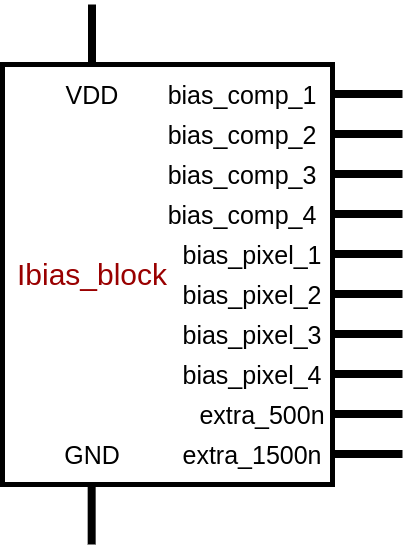
\includegraphics[scale=0.3]{Circuitos/ibias_block_block.png}
    \legend{Fonte: Produzido pelo autor}
\end{figure}
\clearpage
